\chapter{Extension to Maximum Matching}
\label{chap:maximum_matching}

This chapter shows how to extend the perfect matching algorithms to solve the maximum matching problem.

\section{Maximum Matching algorithm}

The extension to maximum matching is based on the following theorem by Lovasz.
\begin{theorem}[\citet{plummer1986matching}]
\label{thm:rank_matching}
    Let \(G\) be a graph and let \(T\) be the Tutte Matrix of \(G\).
    Then, \(\rank(T_G) = 2\nu(G)\).
\end{theorem}

\begin{proof}
  See \citet[p.~560]{Rabin1989}.
\end{proof}

According to \cref{thm:rank_matching}, the number of unmatched vertices can be directly computed as:
\[
    |V(G)| - \rank(T).
\]
To address these unmatched vertices, we can construct an augmented graph by introducing new vertices connected to all existing vertices. 
Specifically, for each unmatched vertex in the original graph, we add a new vertex with connections to every vertex in the original graph. 
This transformation ensures that every previously unmatched vertex now has an adjacent vertex, thus ensuring the existence of a perfect matching.

\newpage
\begin{programruledcaption}{Maximum Matching algorithm}
    \begin{lstlisting}[
      language={pseudocode},
      style=pseudocode,
      style=wider,
      functions={PerfectMatching, TutteMatrix, Rank},
      specialidentifiers={},
    ]
        function MaximumMatching(G)
            $T$ := TutteMatrix(G) // Tutte matrix of \(G\) with random values.
            $G'$ := $G$
            for i := 0; i < |V(G)| - rank(G); i := i + 1 
                $v$ := new vertex
                $V(G')$ := $V(G') \cup \{v\}$
                for $u \in V(G)$ do 
                    $E(G')$ := $E(G') \cup \{uv\}$
            $M'$ := PerfectMatching($G'$)
            $M$ := $\emptyset$
            for $uv \in M'$ do 
                if $u \in E(G)$ and $v \in V(G)$ then // If this edge exists in the original graph.
                    $M$ := $M \cup \{uv\}$
            return M
    \end{lstlisting}
\end{programruledcaption}

\subsubsection{Time complexity}
\noindent
Let \(t(G)\) be the total running time of \(\SC{MaximumMatching}(G)\) and \(f(G)\) be the running time of \(\SC{PerfectMatching}(G)\). Then, we have
\begin{itemize}
\item \textbf{Augmented Graph creation (Lines 4 to 10)}:
The algorithm identifies unmatched vertices and adds corresponding new vertices. 
Since there are at most \(n\) unmatched vertices and each new vertex connects to \(n\) vertices, this phase requires \(O(n^2)\) time;

\item \textbf{Perfect Matching in the augmented graph (Line 11)}: 
The augmented graph has at most \(2n\) vertices. 
By \cref{alg:harvey_complexity}, this step has a time complexity  \(f(G') = O((2n)^\omega) = O(2^\omega n^\omega) = O(n^\omega)\);

\item \textbf{Maximum Matching recovery (Lines 13 to 17)}: 
Checking whether a vertex belongs to the original graph can be implemented in \(O(1)\) time by using integer indexing. 
The overall complexity for this verification across all vertices is \(O(n)\).
\end{itemize}
Combining these steps, the total time complexity is:
\[
t(G) = O(n^2) + f(G') + O(n^2) = O(n^2) + O(n^\omega) + O(n^2) = O(n^\omega). \numberthis \label{alg:maximum_matching_complexity}
\]

\section{Analysis}
\label{Maximum:analysis}
\noindent
This section compares Harvey's algorithm with two maximum matching algorithms:
\begin{enumerate}
   \item The rank-two algorithm described in \cref{alg:rank-two};
   \item A Edmonds-Blossom algorithm implementation made by \citet{giovana:blossom}.
\end{enumerate}
\noindent
The naive algorithm was not compared due to its poor performance.
As a reference, its performance is at least 100 times slower than the Rank-two algorithm in all cases.

\subsection{Methodology}
The comparisons were made through random tests together with a verifier that asserts the output is a valid perfect matching.
For each number of vertices, 10 tests were generated with the following probabilities of an edge being created between every pair of vertices.
\begin{center}
  \begin{tabular}{|c|c|}
    \hline
    Test number & Probability \\
    \hline
    1 & 0.10 \\
    2 & 0.20 \\
    3 & 0.25 \\
    4 & 0.50 \\
    5 & 0.50 \\
    6 & 0.50 \\
    7 & 0.75 \\
    8 & 0.75 \\
    9 & 0.75 \\
    10 & 1.00 \\
    \hline
  \end{tabular}
\end{center}

In total there were 100 different test cases and each test case was executed 50 times to ensure behavior.

\subsubsection{Hardware specifications}

\noindent
The benchmark was executed in a computer with the following specifications:

\begin{center}
  \begin{tabular}{|c|c|}
    \hline
    GPU & GeForce GTX 1660Ti \\
    \hline
    CPU & Intel(R) Core(TM) i7-9750H \\
    \hline
    RAM & 32GB \\ 
    \hline
  \end{tabular}
\end{center}

\subsubsection{Algorithms tested}
The fast matrix multiplication algorithm was \textbf{not} implemented since its threshold is too high for application purposes.
Instead the trivial $O(n^3)$ algorithms was implemented, thus the tested algorithms have the following time complexities, where \(n\) is the number of vertices and \(m\) is the number of edges.
\begin{center}
  \begin{tabular}{|c|c|}
    \hline
    Algorithm & Time complexity \\
    \hline
    Rank-two algorithm & \(O(n^2m + n^3)\) \\
    Harvey's algorithm & \(O(n^3)\) \\
    Edmonds-Blossom algorithm & \(O(n^2m)\) \\
    \hline
  \end{tabular}
\end{center}

\subsection{Results}
\label{results:max_matching}

Figure \cref{fig:max_matching} illustrates the algorithmic performance across test cases. 
The Edmonds-Blossom algorithm demonstrated superior performance compared to the alternative approaches.

\begin{figure}[H]
  \centering
  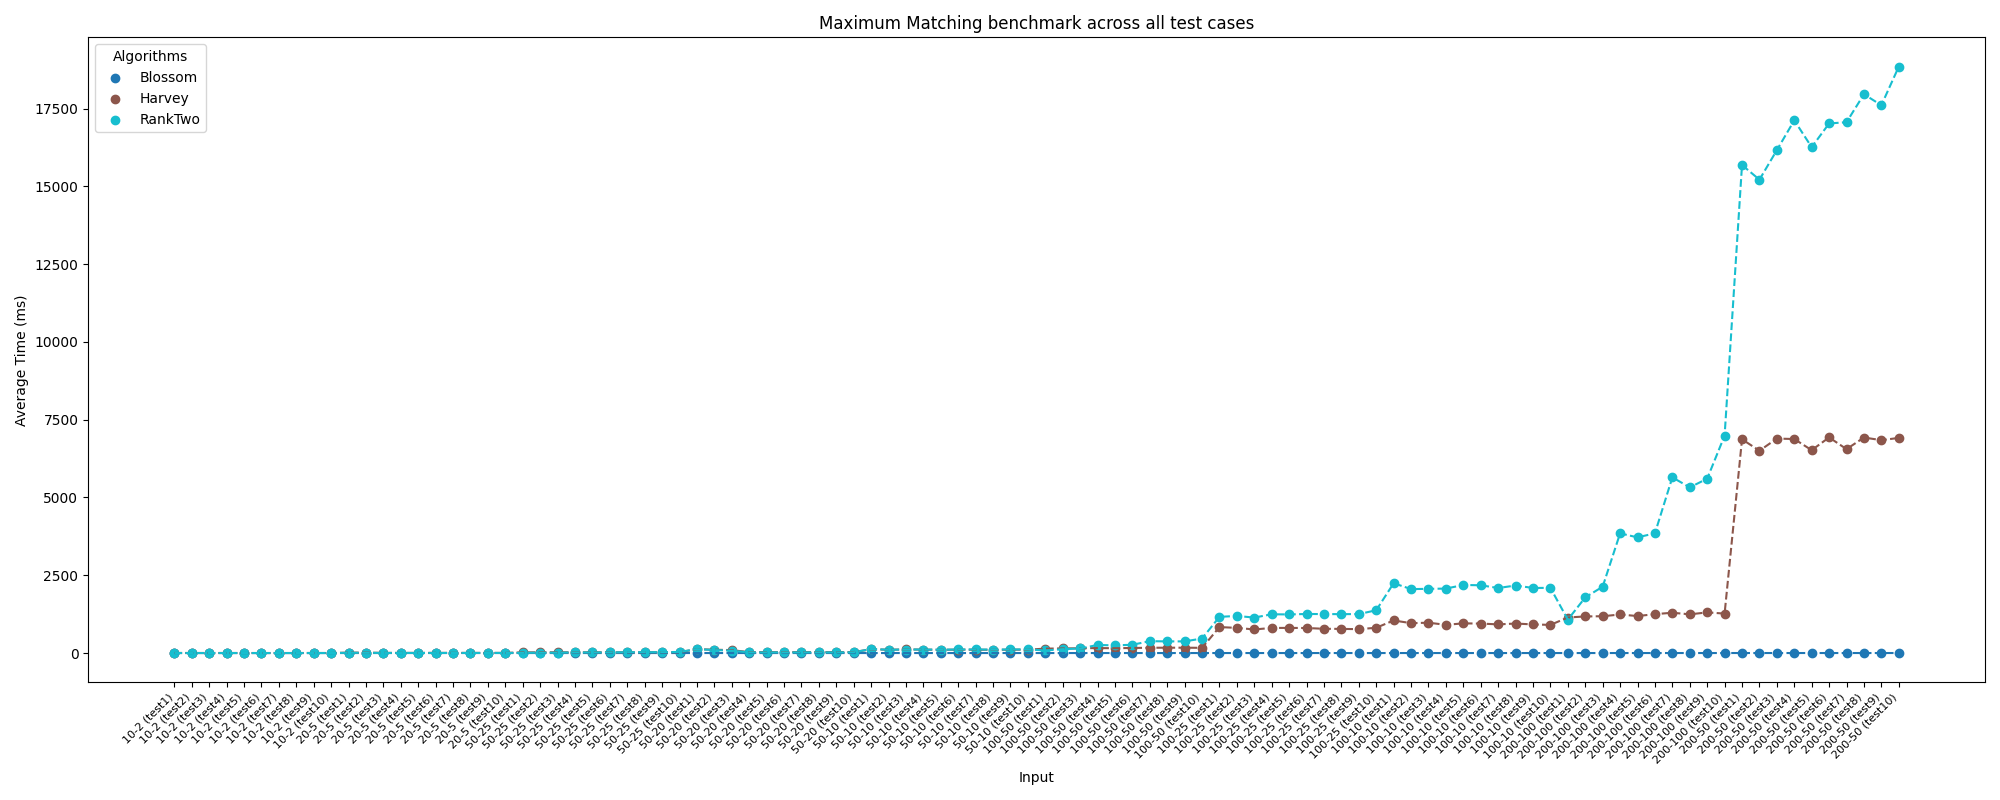
\includegraphics[width=15cm]{maximum_matching_plot.png}
  \caption{Maximum Matching benchmark with all test cases.}
  \label{fig:max_matching}
\end{figure}

Similarly to the perfect matching algorithm, in small graphs (\cref{fig:v10m2-v20m5}) the Rank-two algorithm outperforms the Harvey's algorithm.

\begin{figure}[H]
  \centering
  \begin{subfigure}{.5\textwidth}
    \centering
    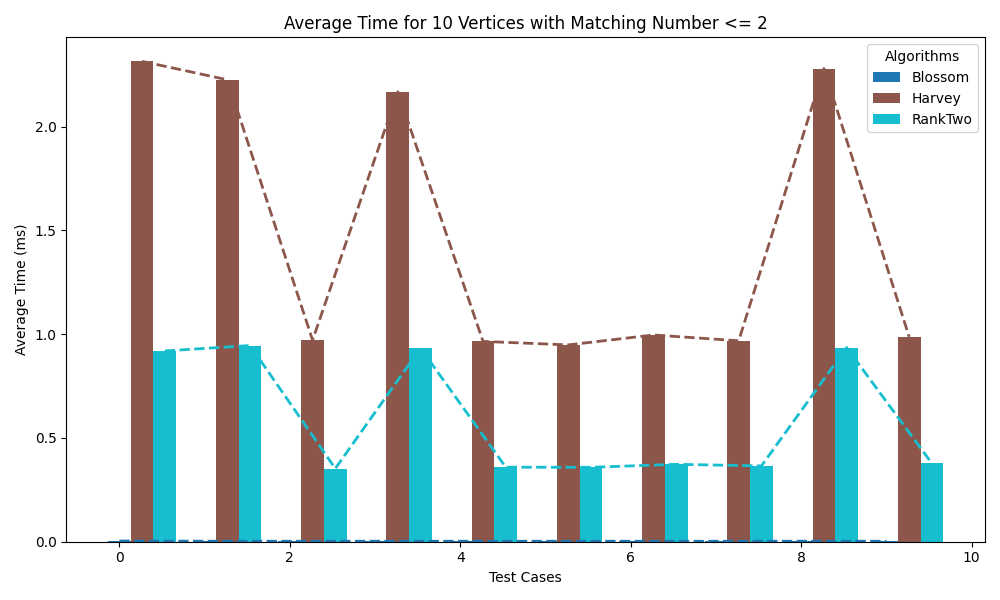
\includegraphics[width=\linewidth]{maximum_matching_v10_m2.png}
  \end{subfigure}%
  \begin{subfigure}{.5\textwidth}
    \centering
    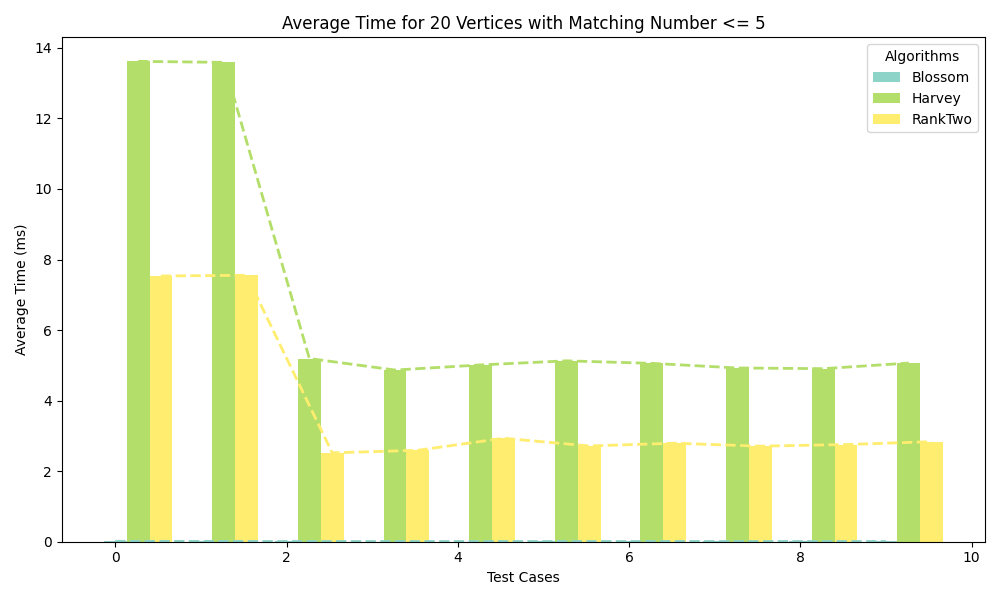
\includegraphics[width=\linewidth]{maximum_matching_v20_m5.png}
  \end{subfigure}
  \caption{Maximum matching benchmark with smaller graphs.}
  \label{fig:v10m2-v20m5}
\end{figure}

In \cref{fig:maxv50}, the impact of matching number on algorithm performance becomes evident through the augmented graph.
The left plot shows both algorithms maintaining stable, similar performance, likely due to the augmented graph's almost doubling the number of vertices.
Conversely, the right plot exhibits behavior reminiscent of the perfect matching algorithm, attributed to fewer added vertices in the augmented graph.

\begin{figure}[H]
  \centering
  \begin{subfigure}{.5\textwidth}
    \centering
    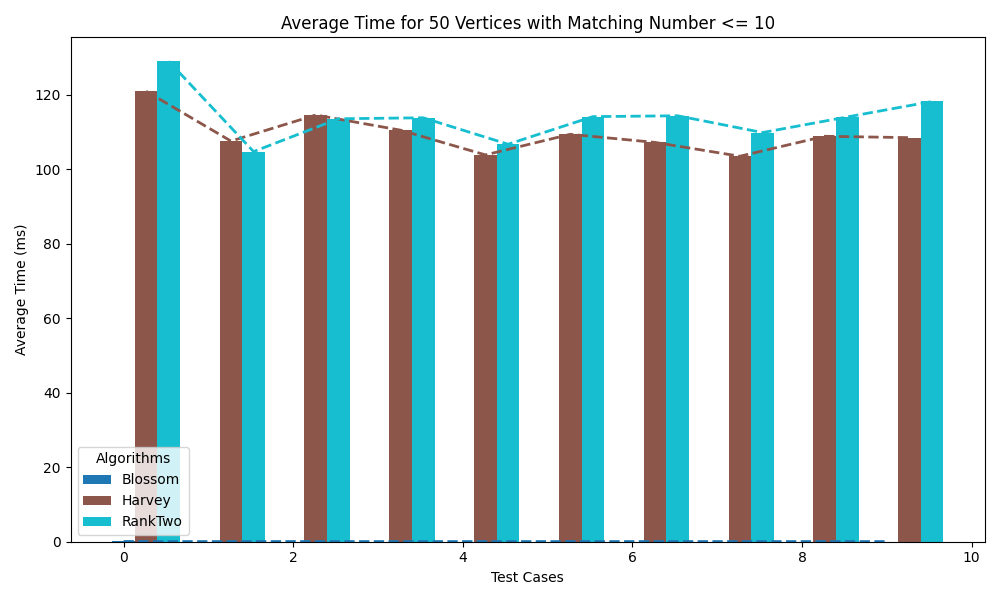
\includegraphics[width=\linewidth]{maximum_matching_v50_m10.png}
  \end{subfigure}%
  \begin{subfigure}{.5\textwidth}
    \centering
    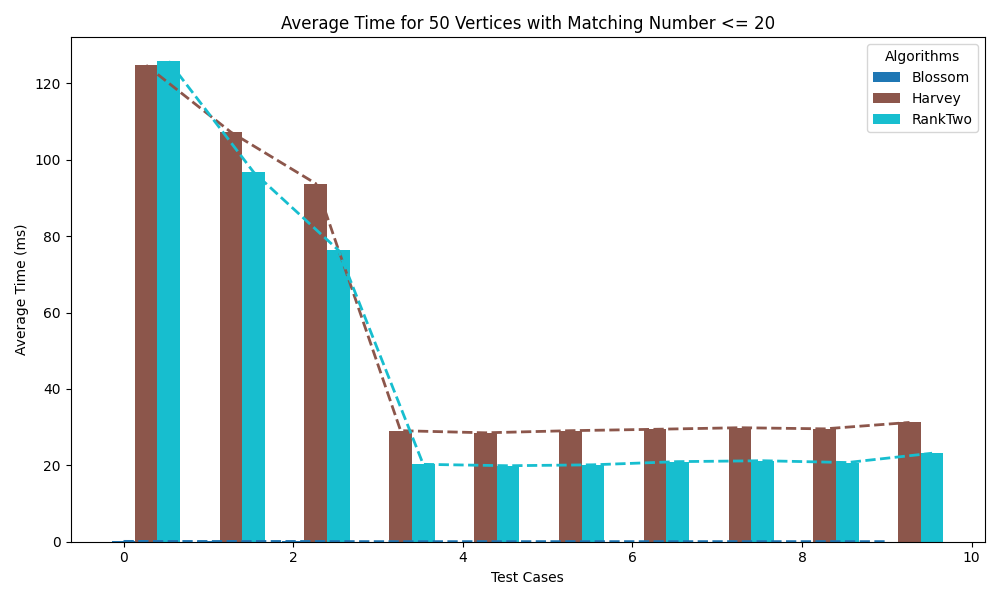
\includegraphics[width=\linewidth]{maximum_matching_v50_m20.png}
  \end{subfigure}
  \caption{Maximum matching benchmark with 50 vertices.}
  \label{fig:maxv50}
\end{figure}


In \cref{fig:maxv100} and \cref{fig:maxv200}, Harvey's algorithm outperforms the Rank-two algorithm.
The performance trend observed in \cref{fig:maxv50} recurs: as the graph's matching number increases, algorithm performance varies significantly due to augmented graph characteristics.

\begin{figure}[h]
  \centering
  \begin{subfigure}{.5\textwidth}
    \centering
    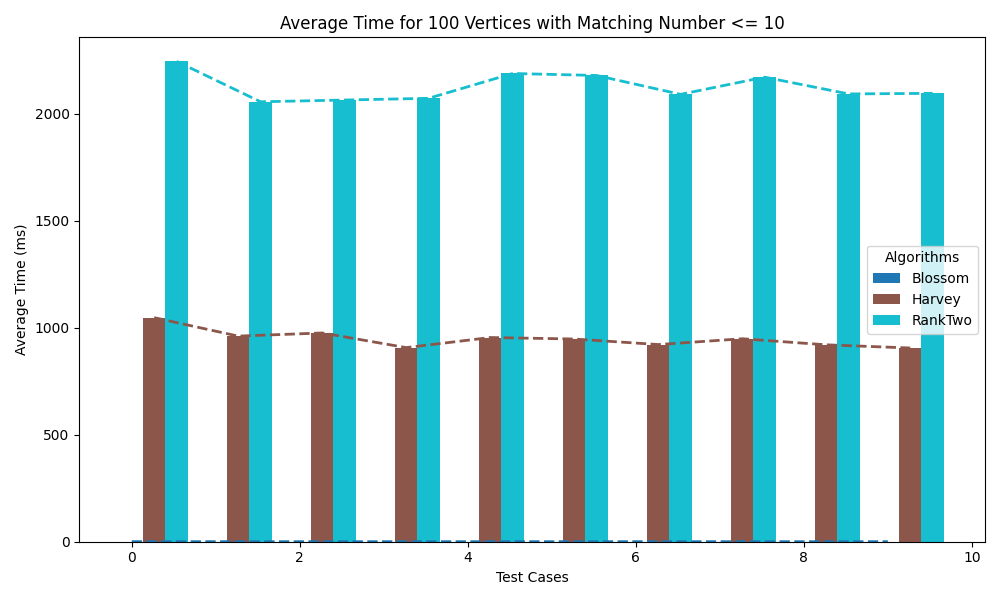
\includegraphics[width=\linewidth]{maximum_matching_v100_m10.png}
  \end{subfigure}%
  \begin{subfigure}{.5\textwidth}
    \centering
    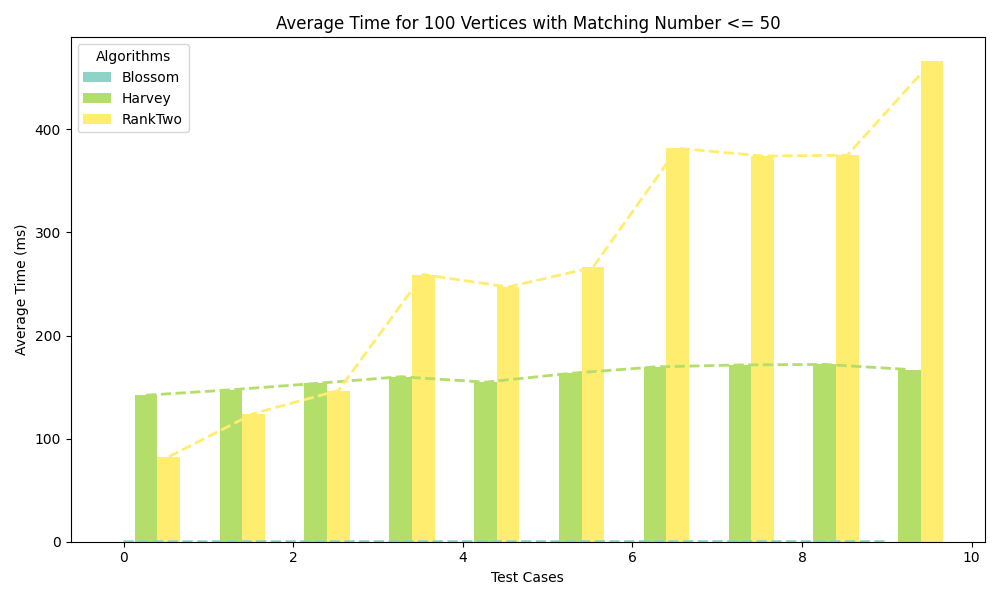
\includegraphics[width=\linewidth]{maximum_matching_v100_m50.png}
  \end{subfigure}
  \caption{Maximum matching benchmark with 100 vertices.}
  \label{fig:maxv100}
\end{figure}

\begin{figure}[h]
  \centering
  \begin{subfigure}{.5\textwidth}
    \centering
    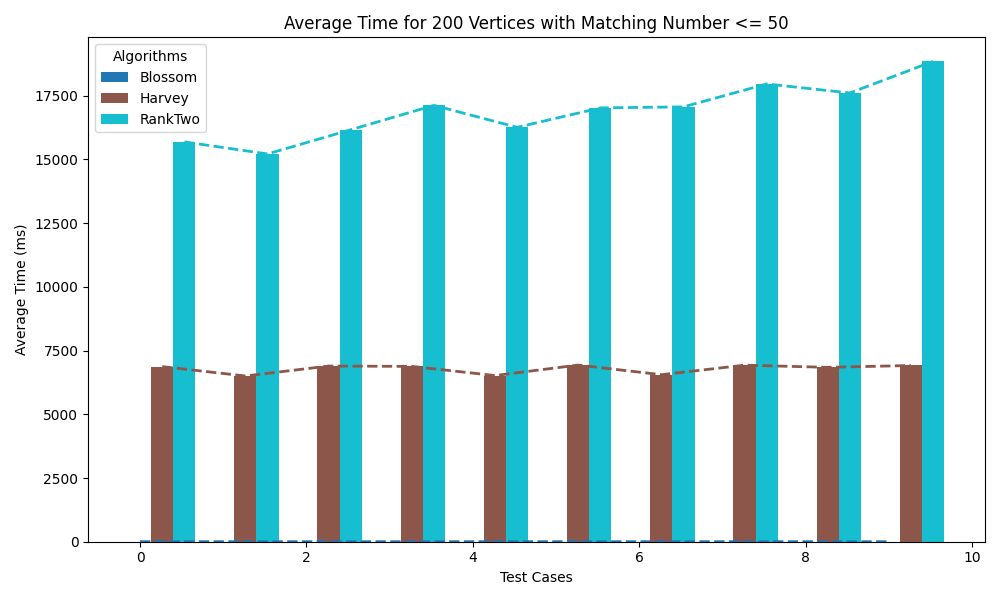
\includegraphics[width=\linewidth]{maximum_matching_v200_m50.png}
  \end{subfigure}%
  \begin{subfigure}{.5\textwidth}
    \centering
    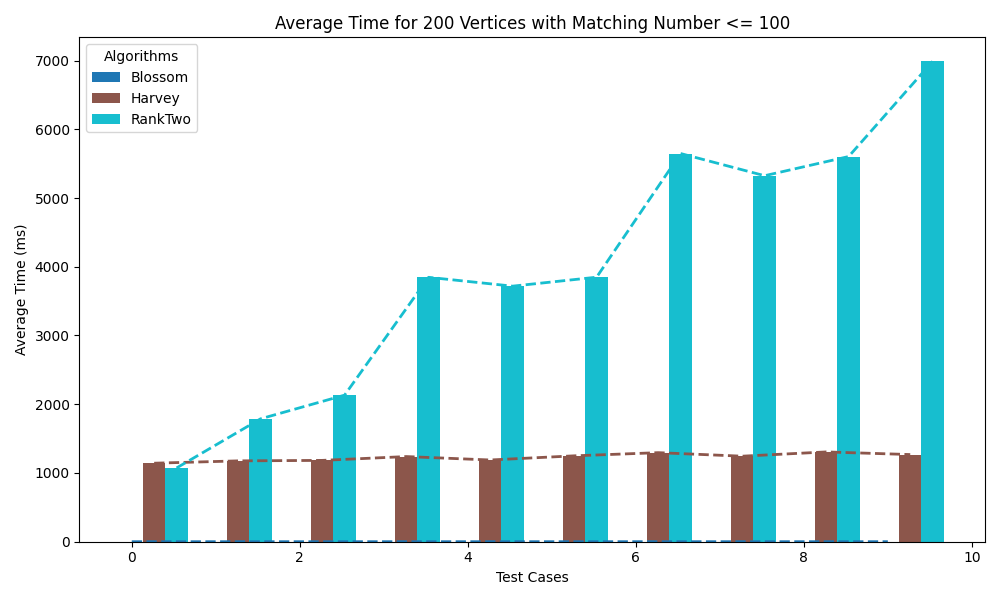
\includegraphics[width=\linewidth]{maximum_matching_v200_m100.png}
  \end{subfigure}
  \caption{Maximum matching benchmark with 200 vertices.}
  \label{fig:maxv200}
\end{figure}

% \begin{figure}[H]
%   \centering
%   \includegraphics[width=12cm]{boxplot_vX_mY.png}
%   \caption{Maximum Matching benchmark with X vertices and matching number Y.}
%   \label{fig:vXmY}
% \end{figure}
